\documentclass[11pt,a4paper]{article}
\usepackage[utf8]{inputenc}
\usepackage{geometry}
\usepackage{graphicx}
\usepackage{booktabs}
\usepackage{caption}
\usepackage{subcaption}
\usepackage{array}
\usepackage{hyperref}
\usepackage{amsmath}
\geometry{margin=1in}

\title{Wildfire Intensity Classification Using Decision Trees, SVMs, and Neural Networks}
\author{Tong Minh Hieu Le}

\begin{document}
\maketitle

\begin{abstract}
This report studies 4 classes about wildfire intensity using satellite-derived and environmental features. Following the assessment requirements, we compare three models covered in Weeks 5--8: a Decision Tree, an SVM, and a Neural Network. The workflow includes exploratory data analysis, preprocessing, tuned hyperparameter, quantitative validation, model comparison, and a final model selection for test-time prediction. The results show that a pruned Decision Tree gives the best validation macro-F1 while remaining interpretable.
\end{abstract}

\section{Introduction}
Wildfire response depends extremely on accurate estimation of fire intensity. Underestimating a fire can delay action and increase harm while overestimating it can waste valuable emergency resources. This makes wildfire intensity classification a practical machine learning task with direct consequences. In this assignment, the goal is to predict the target \texttt{fire\_intensity} with four classes: 0 (Low), 1 (Moderate), 2 (High), and 3 (Extreme), using the provided training and test datasets.

The assignment is suitable for classic supervised learning because the feature set combines numerical and categorical variables, and the test set is drawn from the same operational regions as the training set. The main challenge is not process to unseen countries or regions, but rather class imbalance, missing values, feature types, and the need to compare models with different inductive biases.

\section{A. Task Definition and Dataset Description}
\subsection{Prediction task}
The task is multiclass classification. Each wildfire event must be assigned one of four intensity levels based on environmental and observational features. Since the target is categorical, accuracy alone is not sufficient. Besides, it treats all four classes equally and penalises poor performance on minority classes, we use informative macro-F1.

\subsection{Dataset characteristics}
The dataset contains geographic coordinates (latitude, longitude), temporal information (\texttt{acq\_date}, \texttt{acq\_time}, year, month, season, daynight), location descriptors (region, country), event descriptors (fire\_type, satellite, instrument, confidence), and meteorological/satellite features such as brightness\_k, temp\_max\_c, wind\_max\_kmh, precip\_mm, and humidity\_pct. These variables show both the physical conditions that affect fire spread and the sensing conditions under which events were observed.

The training set is imbalanced, with the Moderate class dominating and the Extreme class being the smallest. This matters because a model that predicts only the majority class can still obtain perfectly decent accuracy while failing in a safety-critical sense. Figure~\ref{fig:classdist} shows that the class frequencies are unequal.

\subsection{Why this dataset is challenging}
The main challenges are:
\begin{itemize}
	\item missing numeric values, which must be imputed without leaking test information;
	\item mixed data types, requiring encoding for categorical variables;
	\item class imbalance, which makes macro-F1 more appropriate than accuracy alone;
	\item non-linear relationships, because fire intensity may depend on interactions between weather, brightness, and location;
	\item limited scope, since the model should be trusted only within the same 7 regions and 35 countries represented in the dataset.
\end{itemize}

\section{B. Exploratory Data Analysis and Data Handling}
\subsection{Exploratory analysis}
Figure~\ref{fig:classdist} shows the class distribution of the training labels. The dataset is imbalanced, but not to the point of making the task trivial. This supports the choice of macro-F1 as the primary evaluation metric. The feature distribution plots in Figures~\ref{fig:dist1} and~\ref{fig:dist2} reveal several important patterns. Brightness\_k is approximately bell-shaped with a noticeable right tail and some outliers. Precip\_mm and wind\_max\_kmh are strongly right-skewed, which suggests that the median is a more robust imputation choice than the mean. Latitude and longitude reflect the multi-region nature of the data rather than a single compact geographic cluster.

The correlation heatmap in Figure~\ref{fig:corr} helps identify redundancy and possible feature interactions. While the correlations are not strong enough to justify aggressive feature removal, they indicate that some variables capture similar signals. The most informative predictors, based on the exploratory correlation analysis and the later tree structure, are brightness\_k, location features, and some weather-related variables. Importantly, not all features need to be individually important for a good model; the value of some features emerges through interactions rather than simple pairwise correlation.

\begin{figure}[ht]
	\centering
	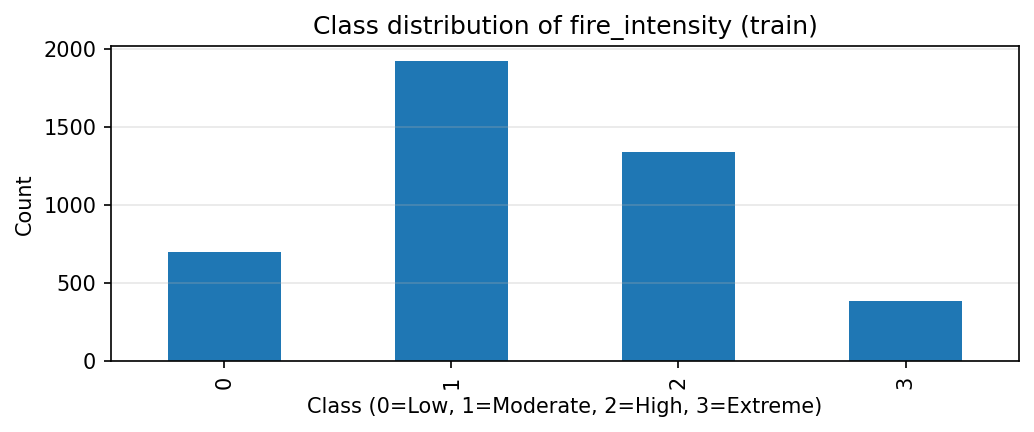
\includegraphics[width=0.75\textwidth]{figures/B_01_class_distribution.png}
	\caption{Training class distribution for \texttt{fire\_intensity}.}
	\label{fig:classdist}
\end{figure}

\begin{figure}[ht]
	\centering
	\begin{subfigure}[b]{0.48\textwidth}
		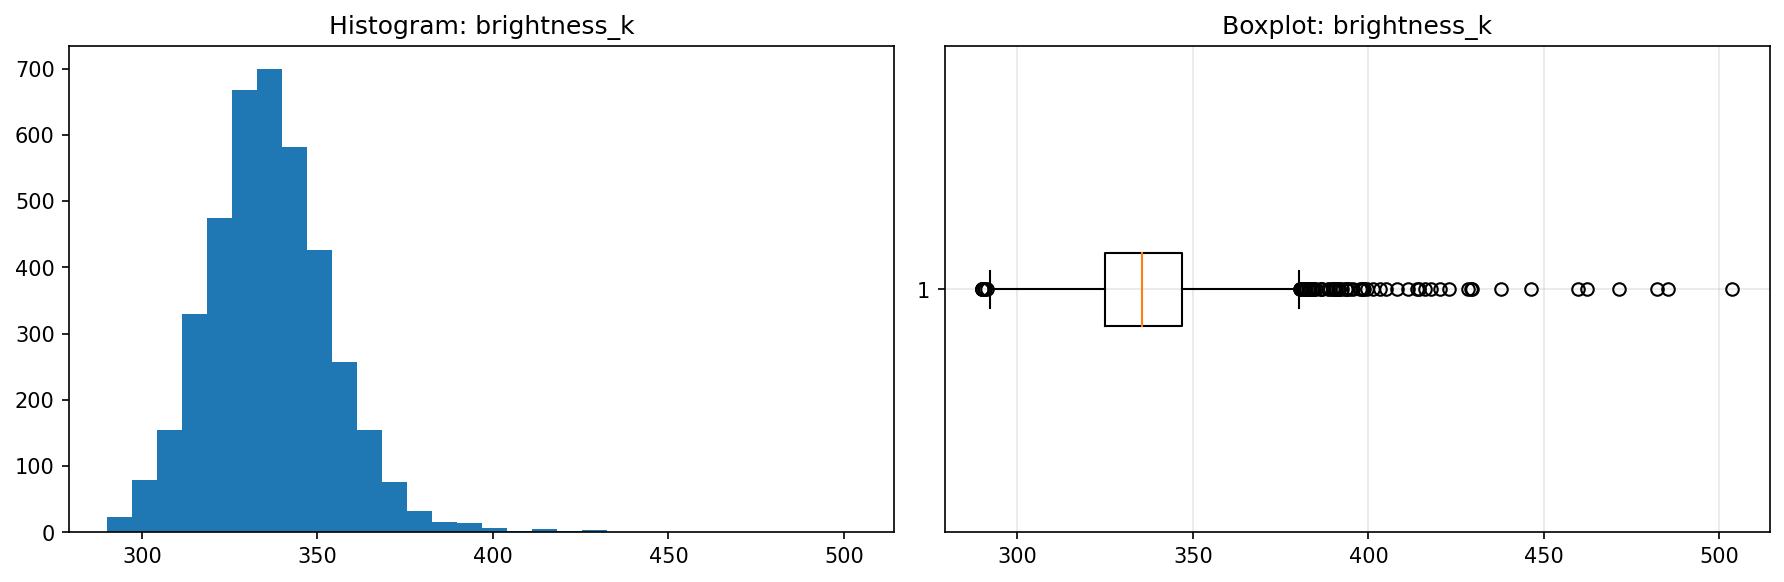
\includegraphics[width=\textwidth]{figures/B_02_brightness_k_distribution.png}
		\caption{Brightness temperature}
	\end{subfigure}
	\begin{subfigure}[b]{0.48\textwidth}
		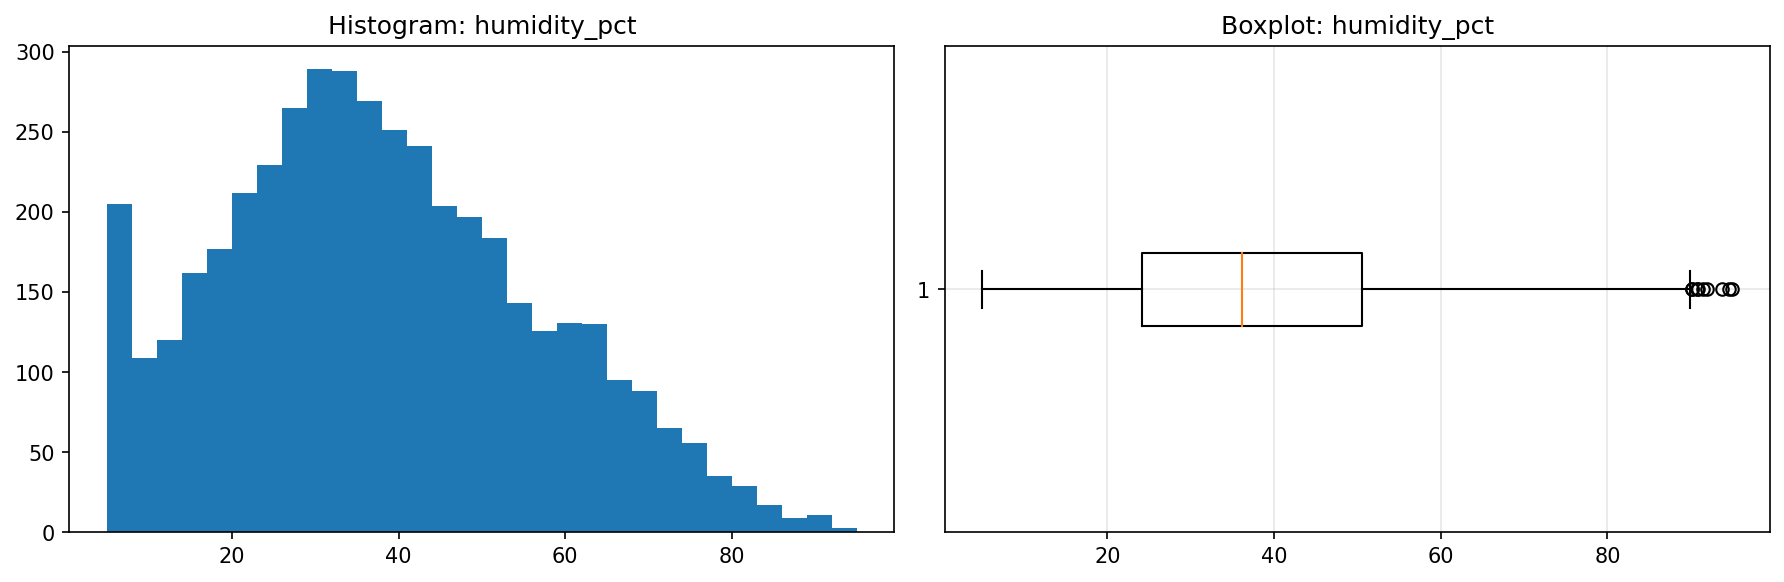
\includegraphics[width=\textwidth]{figures/B_02_humidity_pct_distribution.png}
		\caption{Humidity percentage}
	\end{subfigure}

	\begin{subfigure}[b]{0.48\textwidth}
		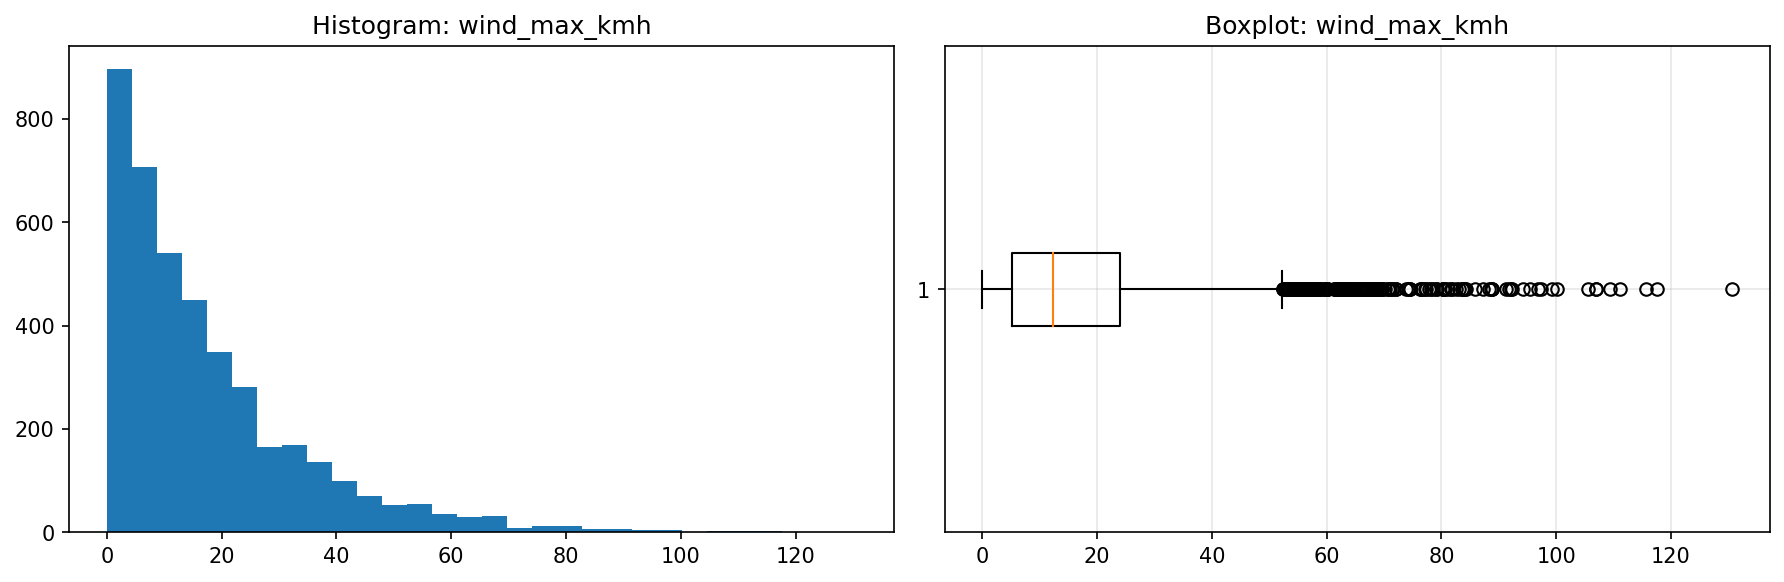
\includegraphics[width=\textwidth]{figures/B_02_wind_max_kmh_distribution.png}
		\caption{Maximum wind speed}
	\end{subfigure}
	\begin{subfigure}[b]{0.48\textwidth}
		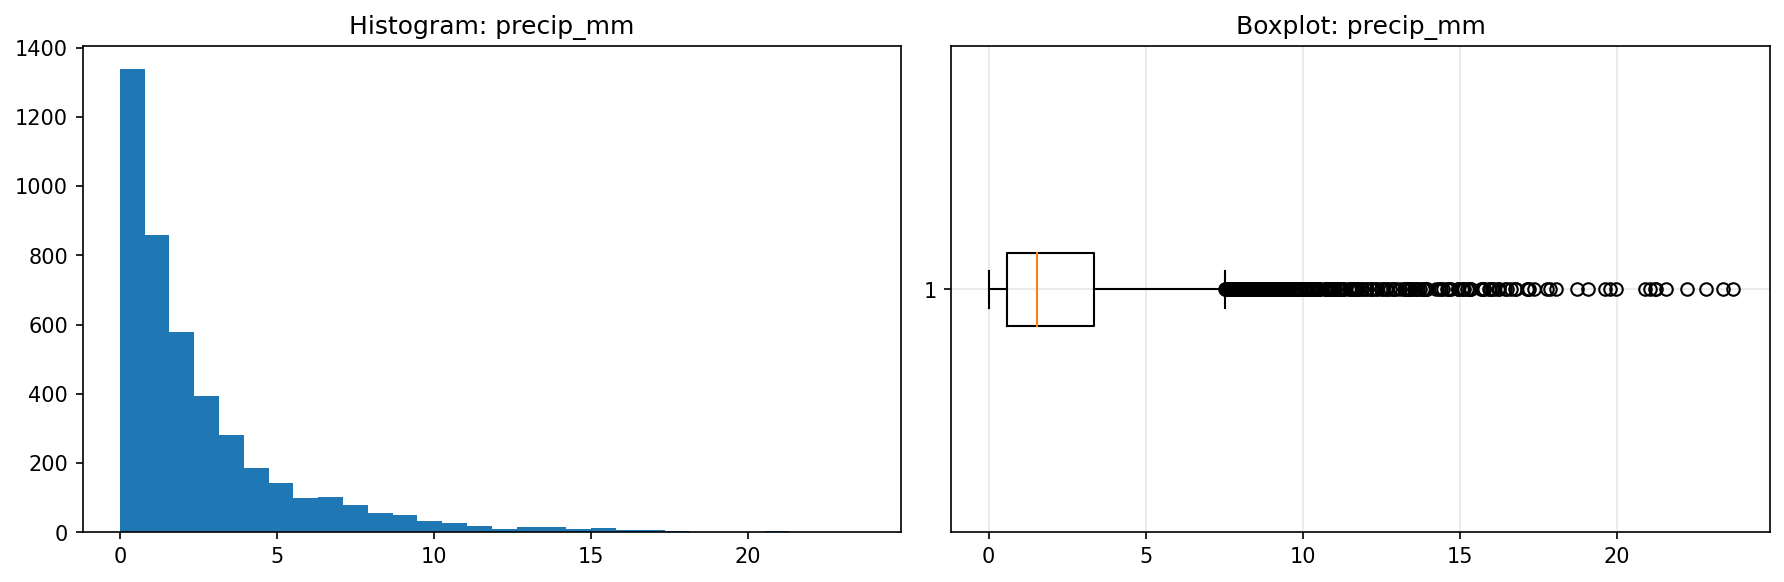
\includegraphics[width=\textwidth]{figures/B_02_precip_mm_distribution.png}
		\caption{Precipitation}
	\end{subfigure}
	\caption{Representative numerical feature distributions. The skewness and outliers motivate median imputation and model scaling.}
	\label{fig:dist1}
\end{figure}

\begin{figure}[ht]
	\centering
	\begin{subfigure}[b]{0.48\textwidth}
		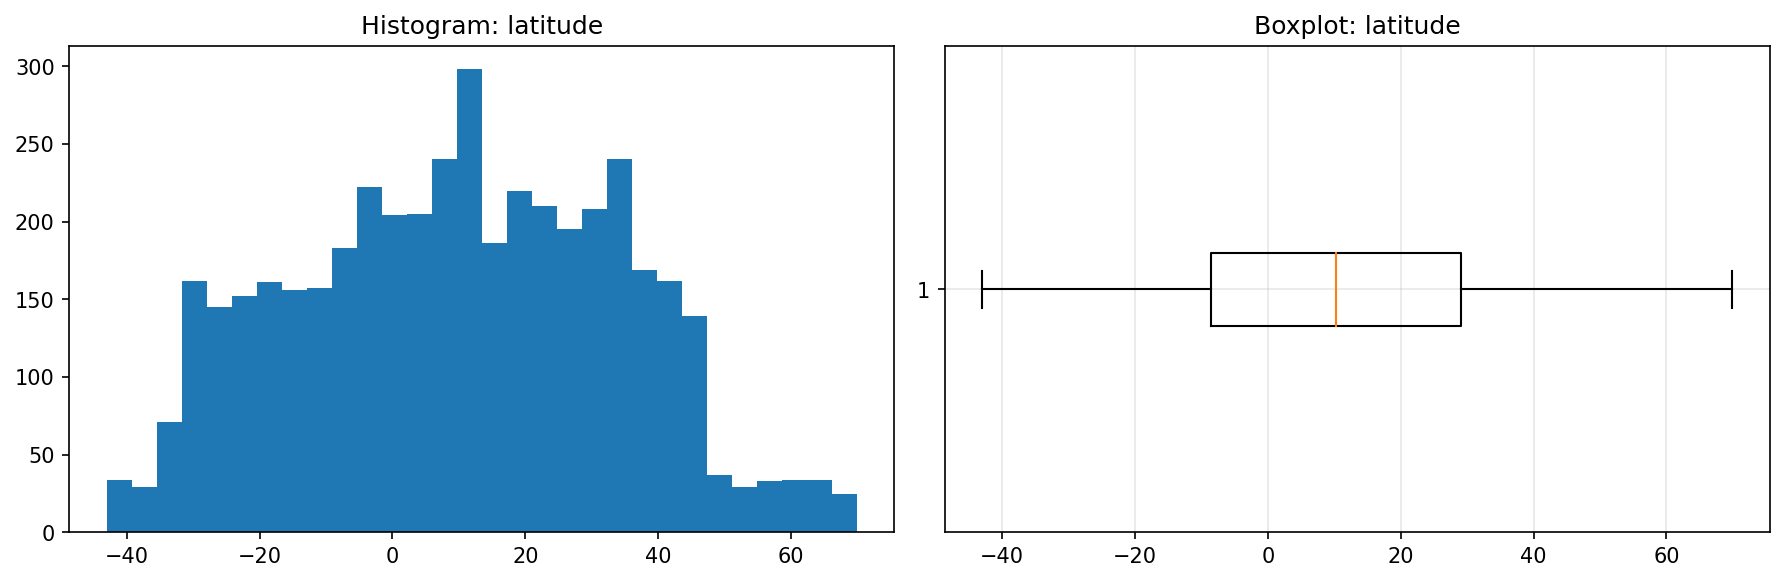
\includegraphics[width=\textwidth]{figures/B_02_latitude_distribution.png}
		\caption{Latitude}
	\end{subfigure}
	\begin{subfigure}[b]{0.48\textwidth}
		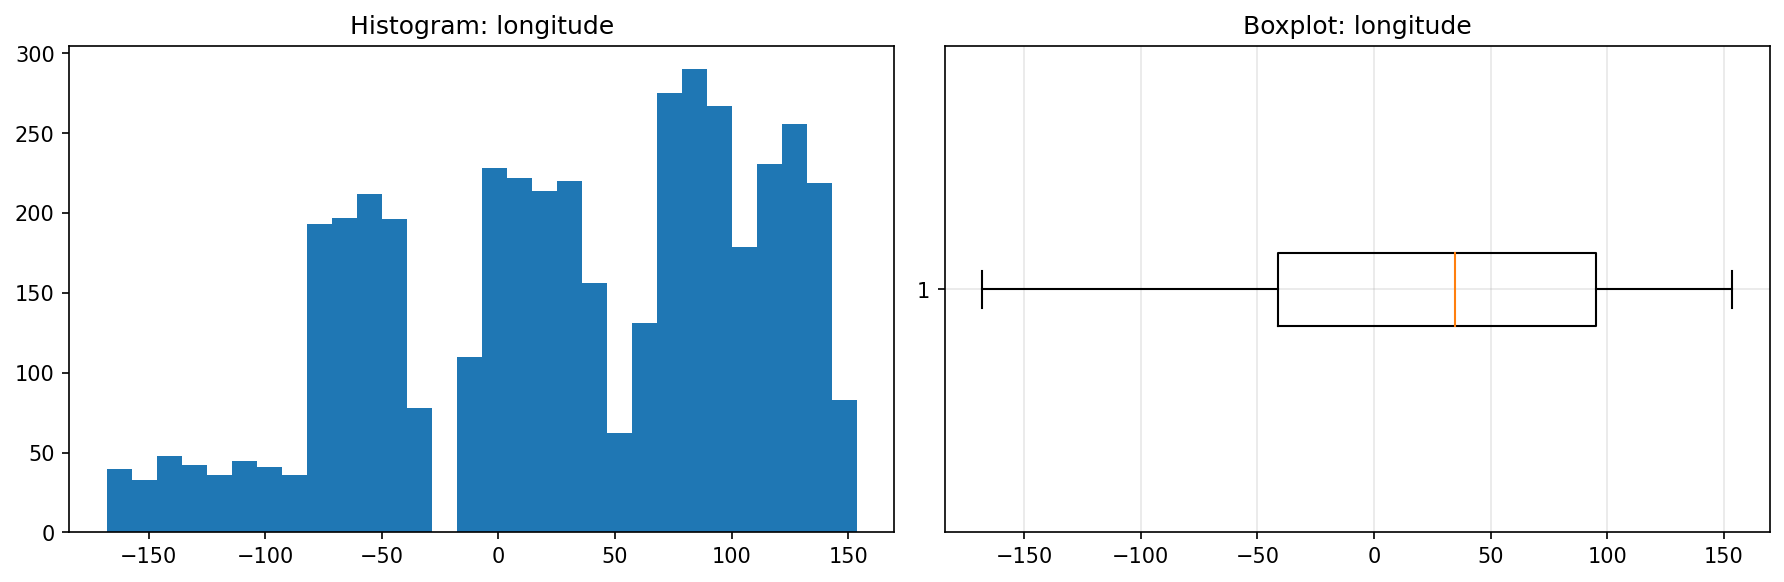
\includegraphics[width=\textwidth]{figures/B_02_longitude_distribution.png}
		\caption{Longitude}
	\end{subfigure}
	\caption{Geographic feature distributions, reflecting the multi-region scope of the dataset.}
	\label{fig:dist2}
\end{figure}

\begin{figure}[ht]
	\centering
	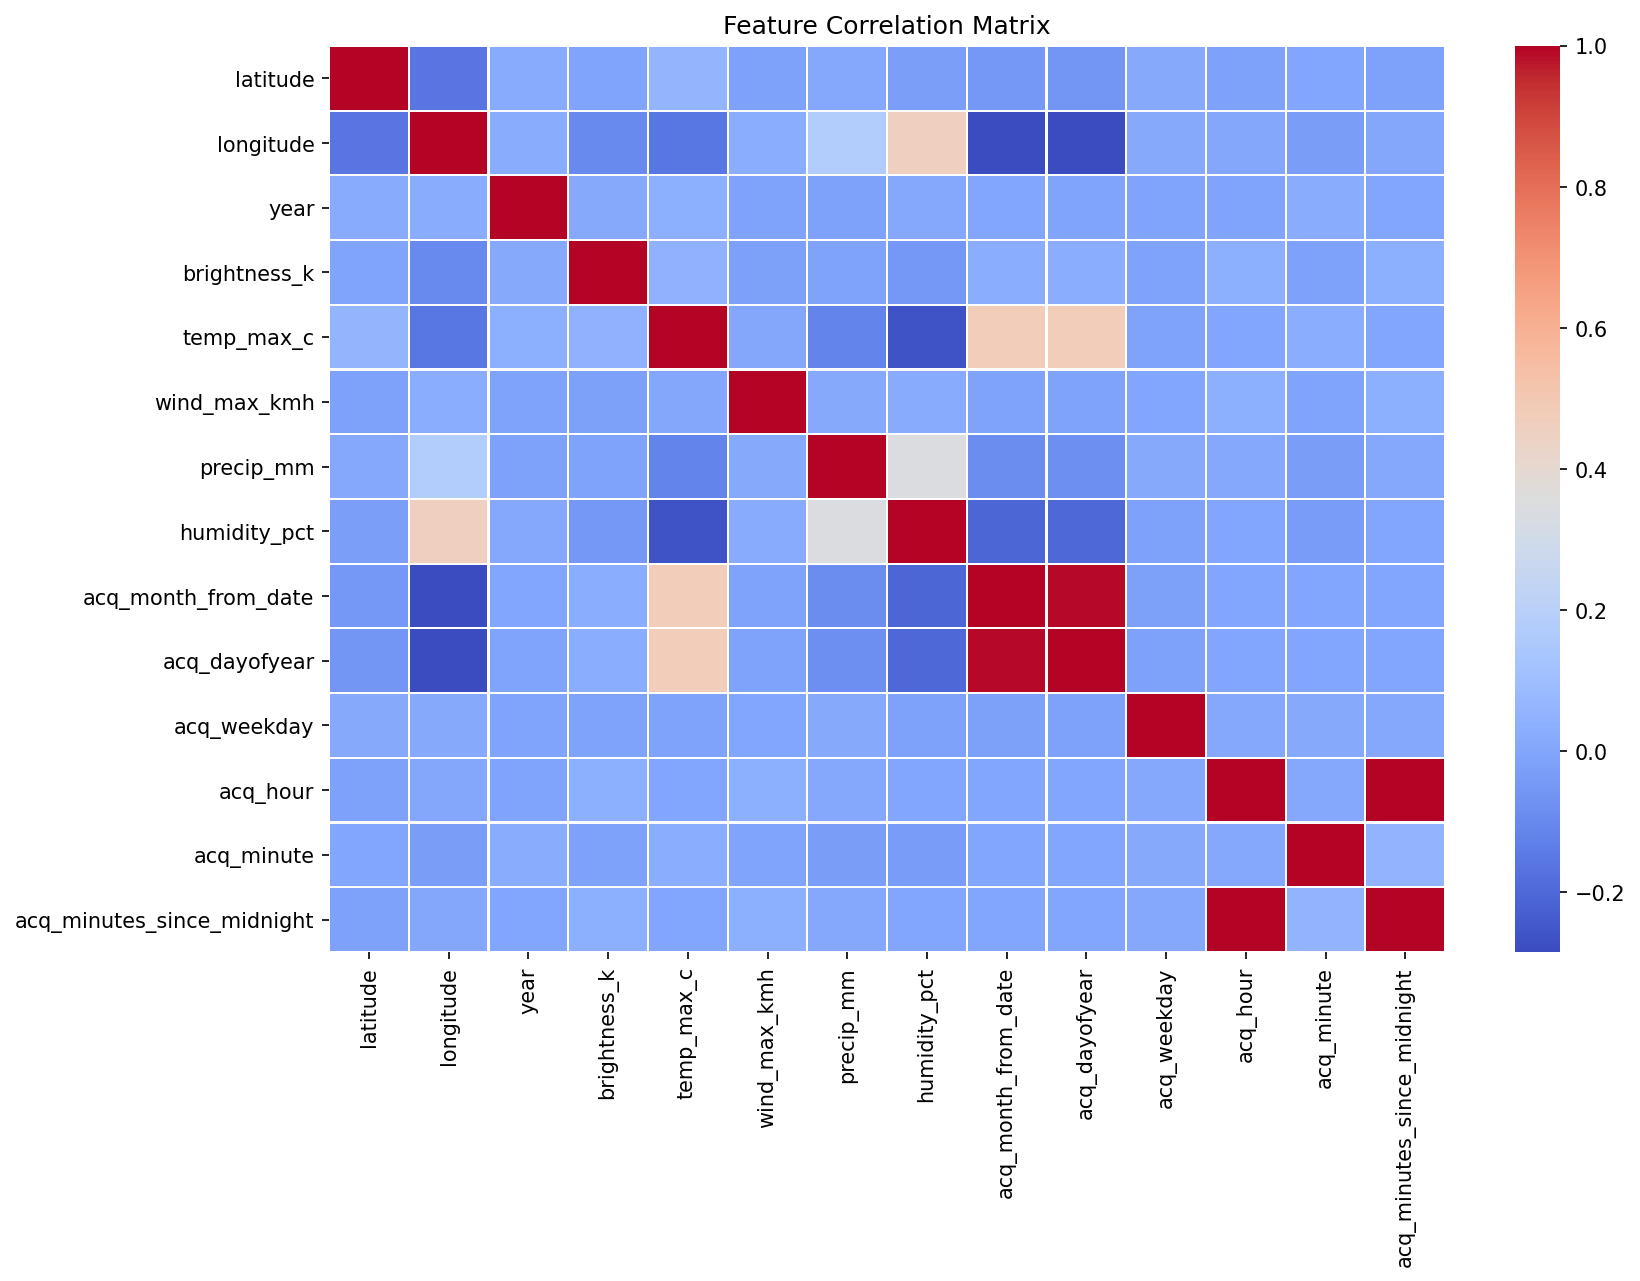
\includegraphics[width=0.8\textwidth]{figures/B_03_correlation_heatmap.png}
	\caption{Correlation heatmap over numerical features. Strong pairwise correlations are limited, suggesting that several features contribute complementary rather than redundant information.}
	\label{fig:corr}
\end{figure}

\subsection{Preprocessing}
All preprocessing steps were performed in a leak-free manner. The training data was split into train, validation, and test partitions using stratified sampling so that the class proportions remained comparable across splits. This is important because macro-F1 is sensitive to minority-class performance, and unstratified splitting could distort the validation estimate.

Missing numeric values were imputed using the median, based on the empirical skewness observed in the EDA. This is a sensible choice because the median is robust to extreme values and does not get pulled by the right tails in wind and precipitation. Categorical variables were one-hot encoded to make them usable by all three model families. Numerical features were scaled with a Min-Max scaler for the SVM and neural network, because both methods are sensitive to feature scale. The Decision Tree was trained on the encoded but unscaled representation, since tree-based methods are scale invariant.

The date and time fields were transformed into more useful numeric variables such as acquisition hour and day-of-year. This preserves temporal information while allowing the models to exploit seasonality and diurnal patterns. Overall, the preprocessing pipeline follows the course material and avoids using methods beyond Week 8.

\section{C. Model Development and Performance Analysis}
\subsection{Evaluation framework}
The evaluation framework consists of a stratified train/validation/test split and two metrics: accuracy and macro-F1. Accuracy is useful for a high-level comparison, but macro-F1 is the main metric because it balances the contribution of each class and is better aligned with the practical cost of failing on rare extreme events. Hyperparameter selection was carried out using validation performance, not test performance, so that the test set remains a genuine final estimate.

\subsection{Decision Tree}
Decision Trees were selected because they are interpretable, handle mixed feature types well after encoding, and naturally capture non-linear interactions through recursive partitioning. Their main weakness is high variance: unconstrained trees tend to overfit, especially on noisy or imbalanced data. That makes them a good candidate for studying the effect of complexity control.

Figure~\ref{fig:dtdepth} shows the effect of \texttt{max\_depth}. As depth increases, training macro-F1 rises rapidly and approaches 1.0, which indicates that the tree can memorise the training set. Validation macro-F1 improves only up to a moderate depth and then plateaus. The gap between training and validation performance is a classic sign of overfitting. This is exactly what theory predicts: deeper trees have lower bias but higher variance.

Figure~\ref{fig:dtprune} shows the effect of cost-complexity pruning via \texttt{ccp\_alpha}. A small amount of pruning improves generalisation by removing weak splits and reducing variance. Strong pruning, however, eventually hurts validation performance because the model becomes too simple and starts to underfit. For COSC2793, this answers the pruning question directly: post-pruning can improve generalisation, but only up to the point where the reduction in variance outweighs the increase in bias.

The visualised tree in Figure~\ref{fig:dttree} provides interpretability. The highest splits are driven by features such as brightness\_k, latitude, longitude, and a small number of weather variables. This suggests that the model is exploiting both the thermal signal and the spatial context. The tree structure also shows that the extreme class is relatively hard to isolate and often appears deeper in the tree, consistent with its lower frequency.

\begin{figure}[ht]
	\centering
	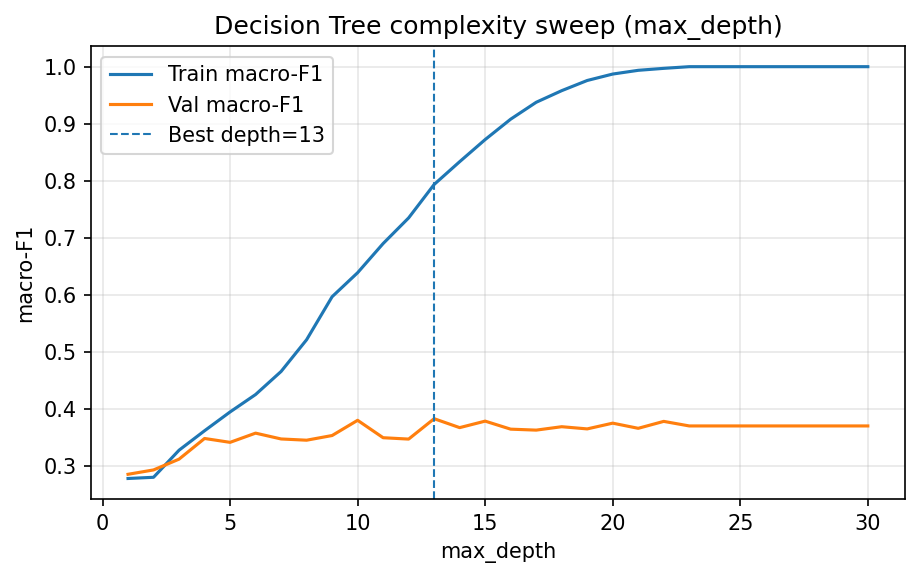
\includegraphics[width=0.78\textwidth]{figures/C1_01_max_depth_sweep.png}
	\caption{Decision Tree complexity sweep over \texttt{max\_depth}. Training performance increases much faster than validation performance, showing overfitting at large depths.}
	\label{fig:dtdepth}
\end{figure}

\begin{figure}[ht]
	\centering
	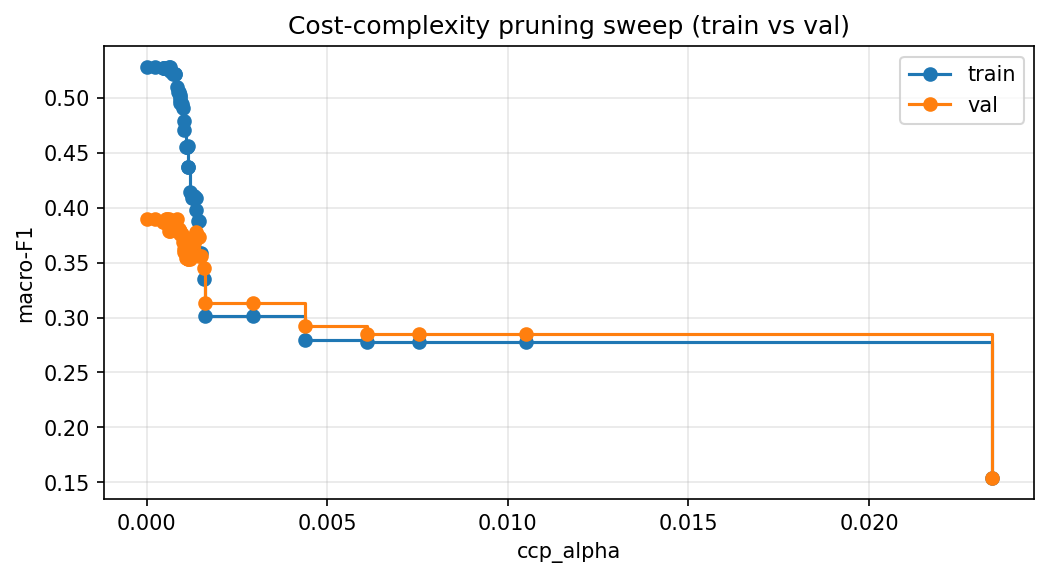
\includegraphics[width=0.78\textwidth]{figures/C1_02_ccp_alpha_pruning.png}
	\caption{Cost-complexity pruning sweep. Moderate pruning improves validation macro-F1, while aggressive pruning underfits.}
	\label{fig:dtprune}
\end{figure}

\begin{figure}[ht]
	\centering
	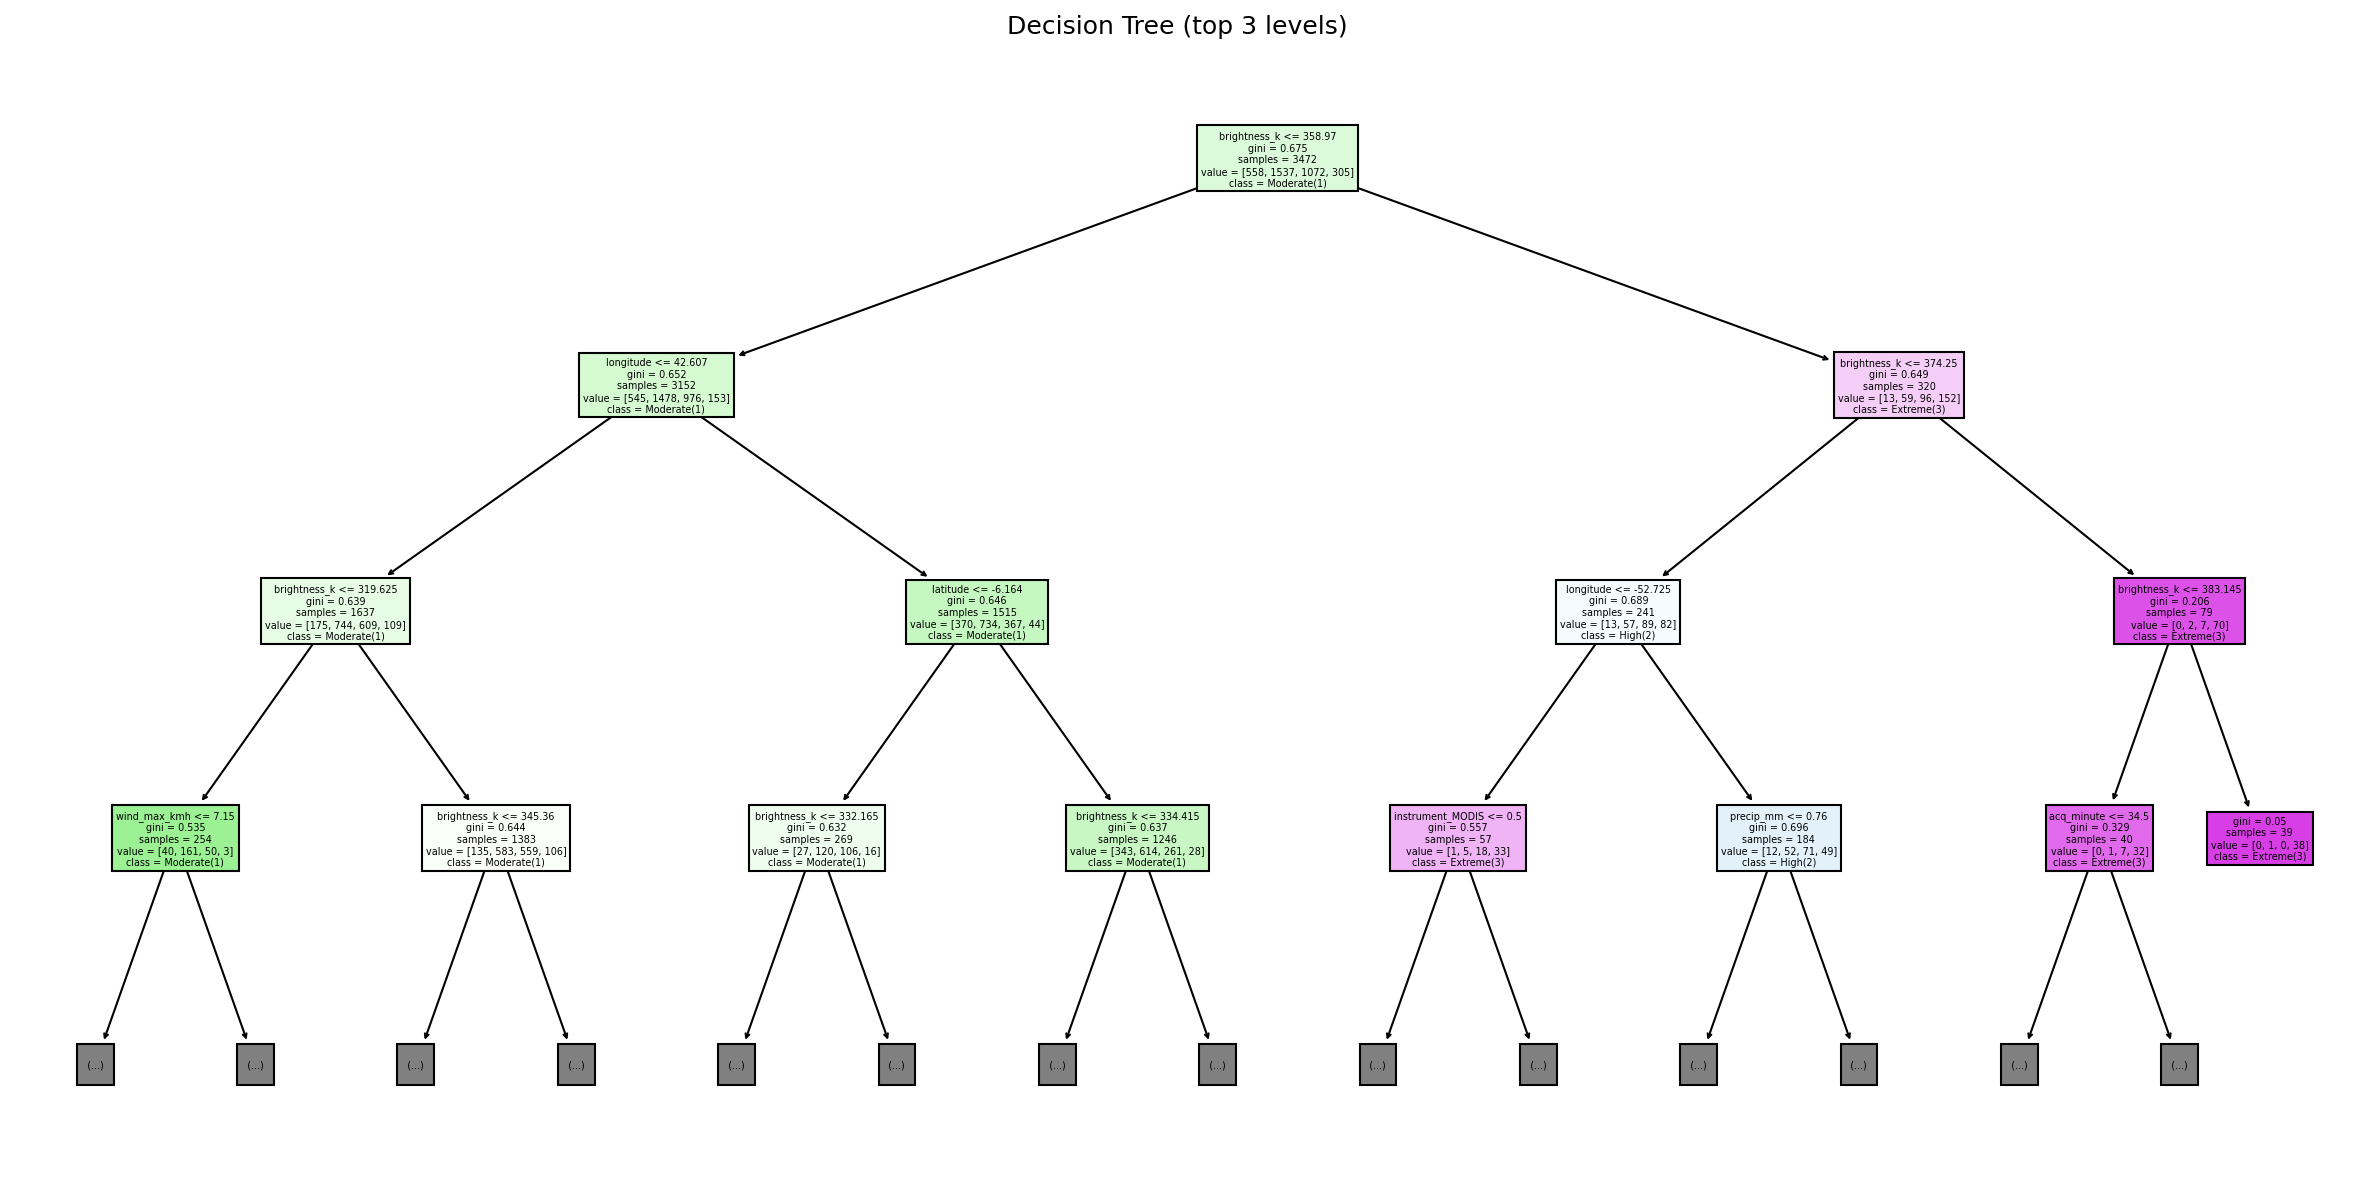
\includegraphics[width=0.92\textwidth]{figures/C1_03_tree_top3_levels.png}
	\caption{Top levels of the final Decision Tree. The tree is interpretable and highlights the most influential feature splits.}
	\label{fig:dttree}
\end{figure}

\subsection{SVM}
SVMs were selected because they are a strong classical baseline for structured data and can model both linear and non-linear boundaries. Their strengths are robust optimisation and good generalisation when the margin is appropriate. Their weaknesses are sensitivity to feature scaling and hyperparameters such as \texttt{C} and \texttt{gamma}. This makes them useful for controlled experiments on model complexity.

Figure~\ref{fig:svmkernel} compares the linear and RBF kernels. The linear kernel produces simpler boundaries and is relatively stable, while the RBF kernel is more flexible but also more sensitive to hyperparameters. In this dataset, the RBF kernel does not dramatically outperform the linear kernel on validation, which suggests that the extra flexibility is not always beneficial once regularisation is considered.

Figure~\ref{fig:svmC} shows the impact of \texttt{C}. Smaller \texttt{C} values impose stronger regularisation and yield smoother decision boundaries with lower training fit but often better generalisation. Larger \texttt{C} values reduce regularisation, increase training macro-F1, and can overfit. Figure~\ref{fig:svmgamma} extends this with \texttt{gamma} for the RBF kernel. A moderate \texttt{gamma} gives the best validation trade-off; too small a value underfits, while too large a value makes the boundary too local and unstable.

The cross-validation search confirmed this behaviour: the best SVM achieved a validation accuracy of 0.4770 and a validation macro-F1 of 0.3688. This is competitive on accuracy, but weaker on macro-F1 than the pruned tree. The confusion matrix in Figure~\ref{fig:svmcm} shows that the SVM tends to predict the middle classes more often and still struggles to isolate Extreme events.

\begin{figure}[ht]
	\centering
	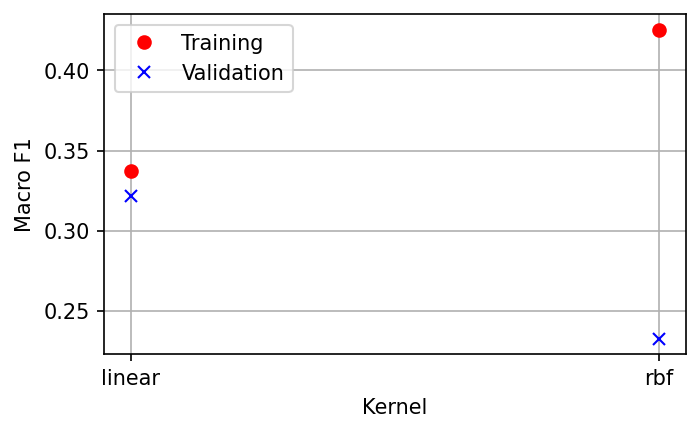
\includegraphics[width=0.46\textwidth]{figures/C2_01_kernel_comparison.png}
	\hfill
	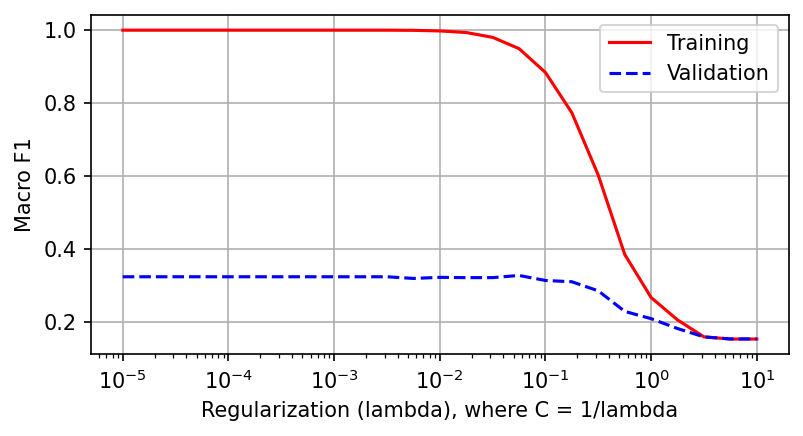
\includegraphics[width=0.46\textwidth]{figures/C2_02_regularization_lambda.png}
	\caption{Kernel comparison and regularisation sweep for SVM. The linear kernel is simpler; the RBF kernel has higher capacity and is more sensitive to regularisation.}
	\label{fig:svmkernel}
\end{figure}

\begin{figure}[ht]
	\centering
	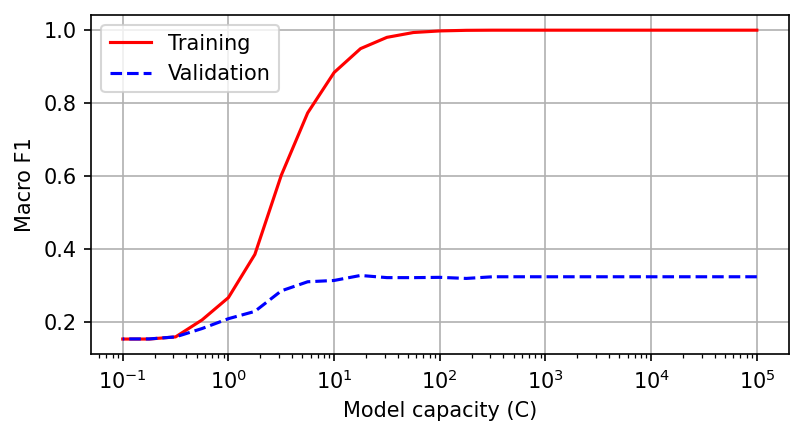
\includegraphics[width=0.78\textwidth]{figures/C2_03_capacity_C.png}
	\caption{Effect of model capacity \texttt{C}. As \texttt{C} increases, training performance rises faster than validation performance, indicating overfitting risk.}
	\label{fig:svmC}
\end{figure}

\begin{figure}[ht]
	\centering
	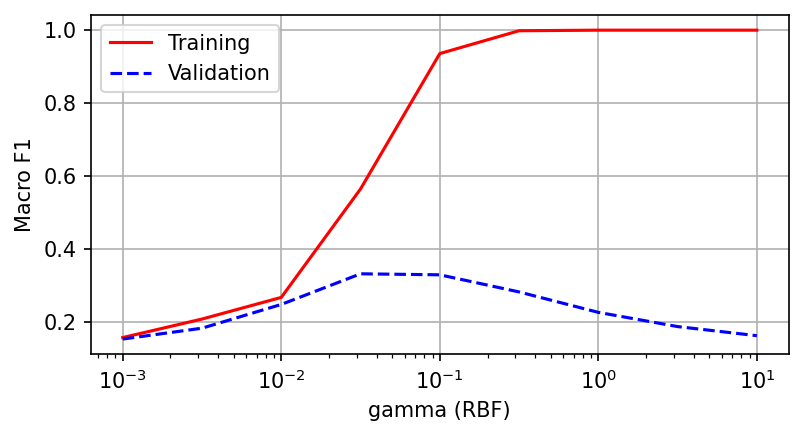
\includegraphics[width=0.78\textwidth]{figures/C2_04_gamma_sweep.png}
	\caption{RBF kernel \texttt{gamma} sweep. Moderate values work best; overly large \texttt{gamma} makes the boundary too complex.}
	\label{fig:svmgamma}
\end{figure}

\begin{figure}[ht]
	\centering
	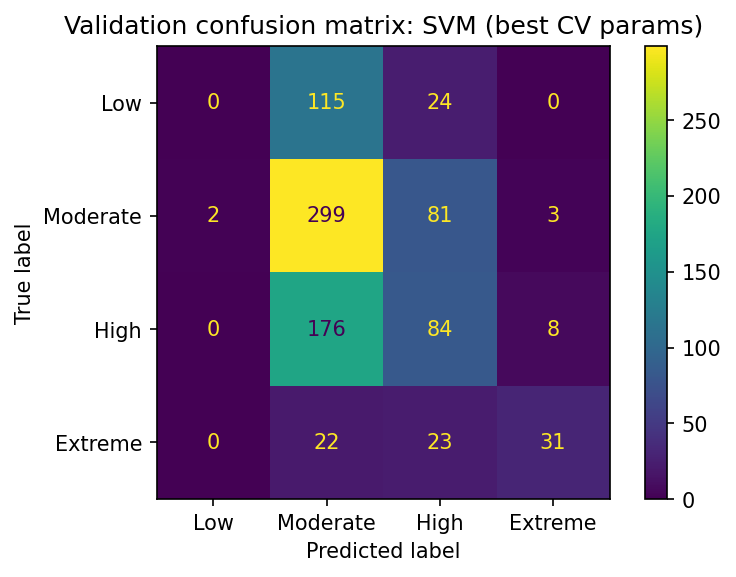
\includegraphics[width=0.62\textwidth]{figures/D_02_confusion_svm_best_cv_params_validation.png}
	\caption{Validation confusion matrix for the tuned SVM. The model separates the classes moderately well, but minority classes remain difficult.}
	\label{fig:svmcm}
\end{figure}

\subsection{Neural Network}
The neural network was selected because the assignment requires a standard feed-forward network and because it can approximate non-linear decision boundaries through learned representations. Its advantages are flexibility and the ability to learn complex feature interactions. Its disadvantages are sensitivity to optimisation settings, longer training time, and lower interpretability.

The learning-rate sweep in Figure~\ref{fig:nnlr} addresses the most important optimisation hyperparameter. A very small learning rate converges slowly and may underfit within the available epoch budget. A very large learning rate causes noisy training and unstable validation curves. In our experiments, the largest learning rate achieved the best validation macro-F1, but the curve is much less stable than the lower-rate runs. This means the optimiser can reach a better solution, but the path is more erratic.

The hidden-size sweep in Figure~\ref{fig:nnhidden} examines model capacity. Larger hidden layers can reduce training loss and improve the best validation score up to a point, but beyond that the gains are limited and the network becomes harder to train reliably. This is consistent with the bias--variance trade-off and with the expected effect of hidden width on function class complexity. The training curves show that the network is not simply benefiting from more parameters; optimisation quality and generalisation also matter.

The neural network achieved the same validation accuracy as the tuned SVM (0.4770) but a lower validation macro-F1 (0.3457). The confusion matrix in Figure~\ref{fig:nncm} indicates that the model over-predicts the majority classes and struggles most with Extreme events. This is not surprising: with only a shallow architecture and limited data, the network may not extract class-discriminative structure better than the tree.

\begin{figure}[ht]
	\centering
	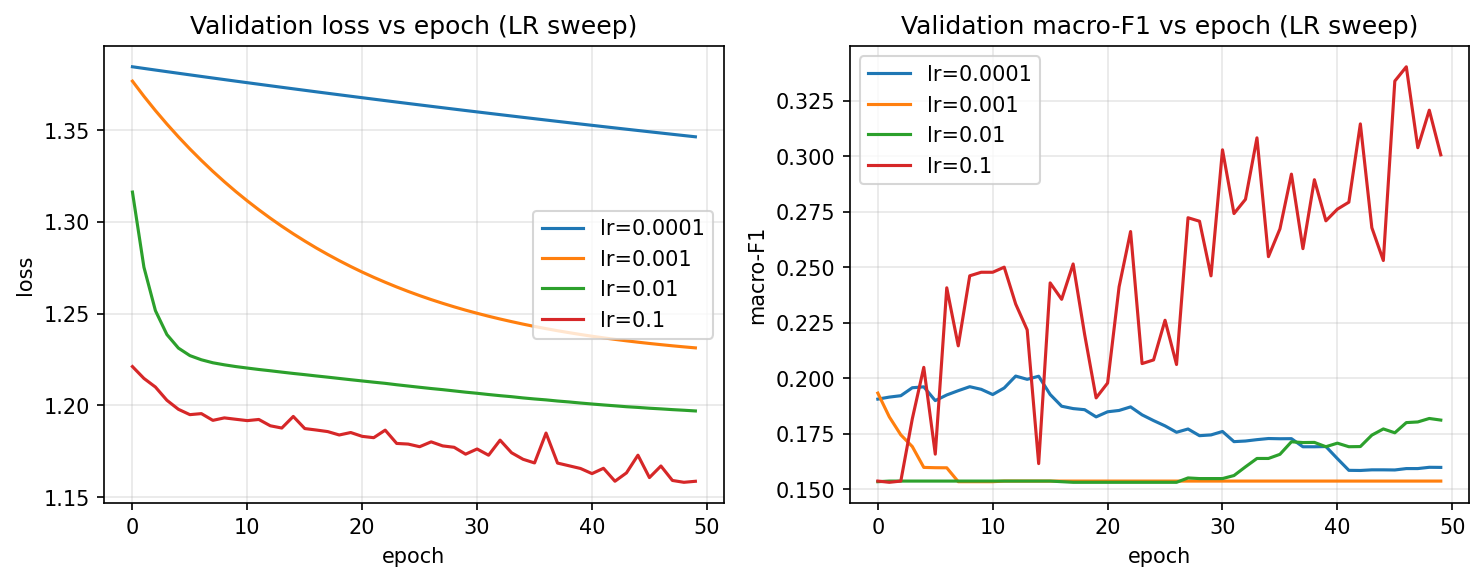
\includegraphics[width=0.95\textwidth]{figures/C3_01_lr_sweep.png}
	\caption{Learning-rate sweep for the neural network. Stable convergence depends strongly on the step size.}
	\label{fig:nnlr}
\end{figure}

\begin{figure}[ht]
	\centering
	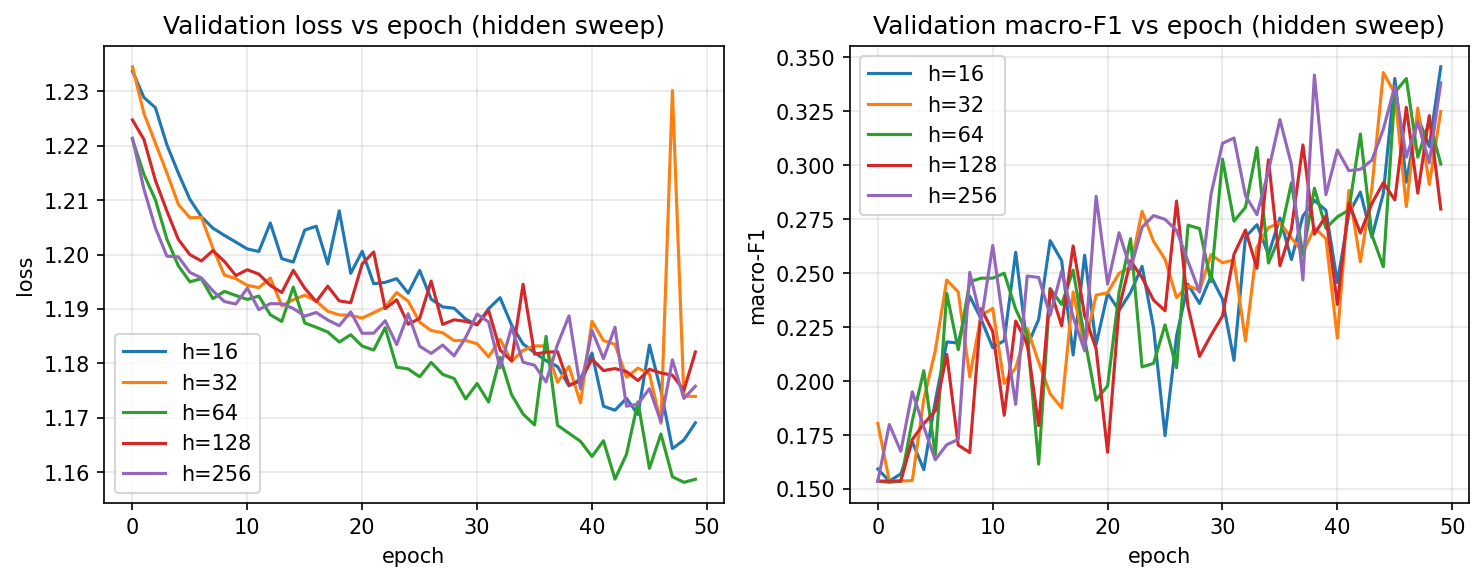
\includegraphics[width=0.95\textwidth]{figures/C3_02_hidden_sweep.png}
	\caption{Hidden-size sweep for the neural network. Wider networks improve capacity, but validation gains saturate.}
	\label{fig:nnhidden}
\end{figure}

\begin{figure}[ht]
	\centering
	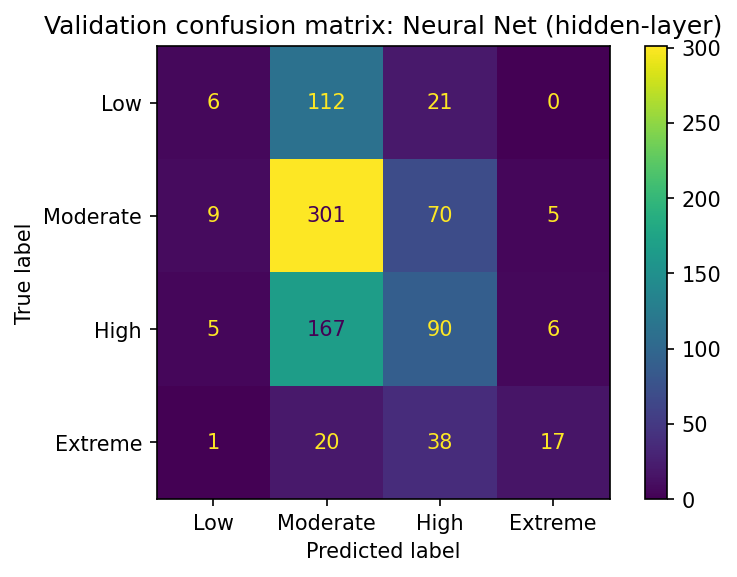
\includegraphics[width=0.60\textwidth]{figures/D_03_confusion_neural_net_hidden-layer_validation.png}
	\caption{Validation confusion matrix for the neural network. The model is less balanced than the pruned tree.}
	\label{fig:nncm}
\end{figure}

\section{D. Model Comparison}
Table~\ref{tab:compare} summarises the validation results. The pruned Decision Tree is the strongest model in terms of macro-F1, which is the more appropriate metric here. SVM and the neural network tie on accuracy, but both fall behind on macro-F1. This indicates that more complex models do not automatically win: the best model is the one that balances bias, variance, regularisation, and the structure of the available data.

\begin{table}[ht]
\centering
\begin{tabular}{lcc}
\toprule
Model & Validation Accuracy & Validation Macro-F1 \\
\midrule
Decision Tree (pruned) & 0.4343 & 0.3899 \\
SVM (best CV params) & 0.4770 & 0.3688 \\
Neural Network (hidden-layer) & 0.4770 & 0.3457 \\
\bottomrule
\end{tabular}
\caption{Validation performance comparison. Macro-F1 is the main criterion because it reflects balanced performance across all classes.}
\label{tab:compare}
\end{table}

\begin{figure}[ht]
	\centering
	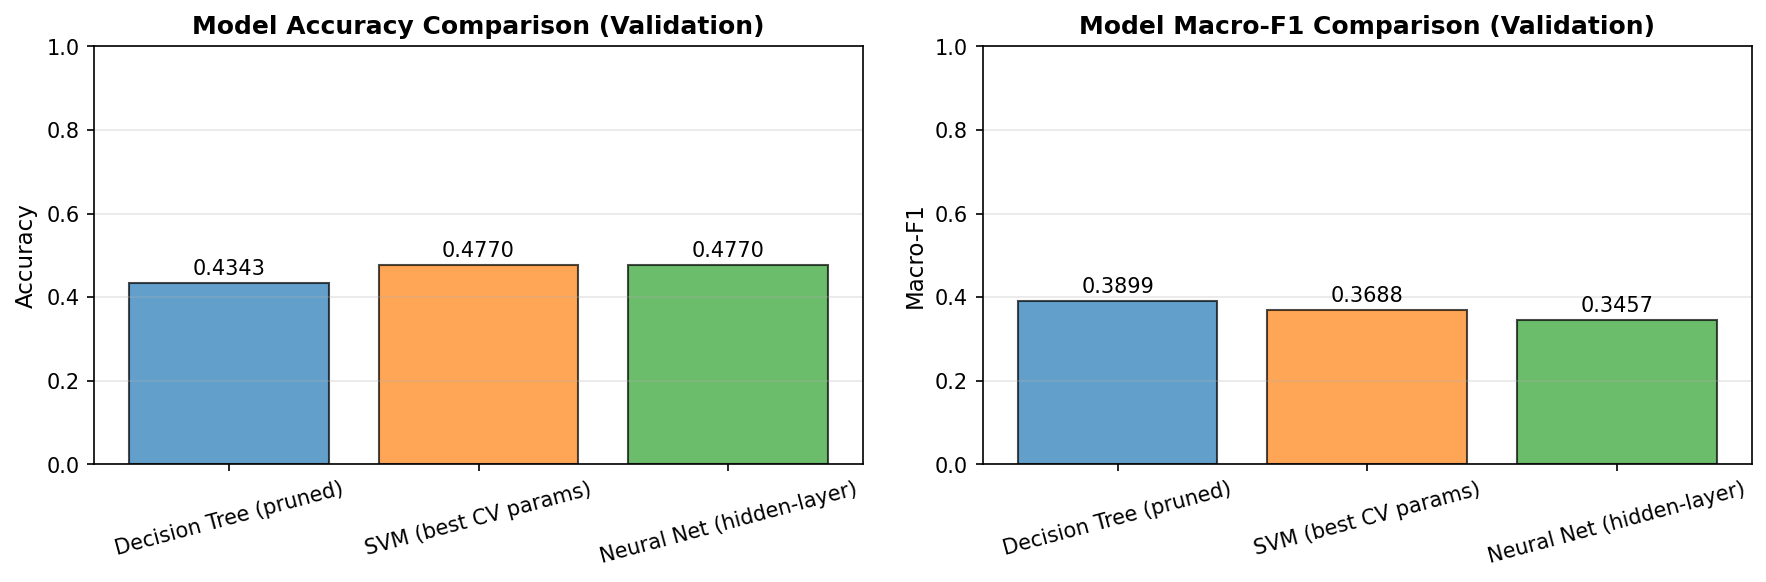
\includegraphics[width=0.95\textwidth]{figures/D_00_model_performance_comparison.png}
	\caption{Validation performance comparison. The pruned Decision Tree has the highest macro-F1.}
	\label{fig:comp}
\end{figure}

The models differ in how they separate classes. The Decision Tree creates axis-aligned, piecewise-constant regions, so it is the easiest to interpret and the most stable after pruning. The linear SVM gives a simpler global boundary, while the RBF SVM produces more complex non-linear decision regions and is therefore more sensitive to regularisation. The neural network also learns non-linear boundaries, but its training behaviour is especially sensitive to the learning rate and hidden size. In this task, increased complexity does not guarantee better generalisation because the available features already contain strong structured signals, and the class imbalance rewards models that avoid overfitting the majority class.

The experimental results are consistent with theory. Higher-capacity models fit the training data better, but the simpler pruned tree generalises best on macro-F1. This is exactly what the bias--variance trade-off predicts: reducing complexity and using regularisation can improve out-of-sample performance when the dataset is noisy, finite, and class imbalanced.

\section{E. Final Model Selection, Justification, and Evaluation}
The final model is the pruned Decision Tree. It was selected because it achieved the best validation macro-F1, it remains interpretable, and its decisions can be explained in terms of meaningful environmental variables. In an emergency-response setting, interpretability is valuable because it allows analysts to sanity-check the model and understand why a particular event was predicted as more intense.

To obtain the test results, the selected tree was refit on the combined training and validation data and then evaluated on the held-out test set. The test confusion matrix is shown in Figure~\ref{fig:testcm}. This preserves the integrity of the validation process while still making use of all labelled development data for the final model. The saved test predictions are then exported in the required submission format.

\begin{figure}[ht]
	\centering
	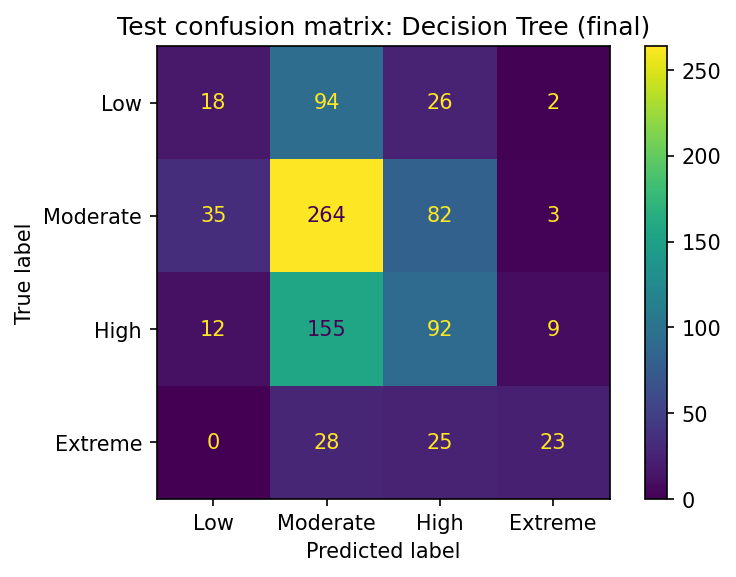
\includegraphics[width=0.60\textwidth]{figures/E_01_confusion_decision_tree_test.png}
	\caption{Test confusion matrix for the final pruned Decision Tree.}
	\label{fig:testcm}
\end{figure}

Beyond performance, the pruned tree is preferred because it is easier to deploy, easier to explain, and less fragile than the neural network or an aggressively tuned SVM. For a high-impact application such as wildfire response, a slightly simpler but more transparent model is often the better professional choice.

\section{F. Ethical Considerations and Professional Responsibilities}
This task has clear ethical dimensions because predictions may influence resource allocation, emergency prioritisation, and potentially public safety decisions. A model that systematically underestimates extreme events could contribute to harm, while a model that overestimates low-risk events could waste resources. This makes class imbalance and minority-class performance especially important.

Professional responsibilities include documenting the preprocessing and model-selection process, reporting metrics honestly, and clarifying the model's limits. The model should not be presented as a substitute for expert judgment. It is trained only on the regions and countries represented in the dataset, so it should not be assumed to generalise to entirely different geographies or sensing conditions without further validation. Human-in-the-loop oversight is therefore essential.

\section{G. Conclusion}
This assignment demonstrates a complete supervised learning workflow for wildfire intensity classification. The EDA identified class imbalance and skewed variables, the preprocessing pipeline handled missing values and categorical encoding in a leak-free way, and the three models were compared using controlled experiments. The pruned Decision Tree achieved the best validation macro-F1 and offered the best balance of performance, robustness, and interpretability. The results show that more complex models do not always perform better; model choice must reflect the data, the evaluation metric, and the operational context.

\section{H. References}
\begin{thebibliography}{9}
\bibitem{sklearn} scikit-learn developers, \emph{scikit-learn user guide}, \url{https://scikit-learn.org/}.
\bibitem{pytorch} PyTorch contributors, \emph{PyTorch documentation}, \url{https://pytorch.org/docs/}.
\bibitem{course} COSC2793 Computational Machine Learning lecture slides and lab materials, Weeks 5--8.
\bibitem{dataset} Alitaqishah, \emph{Wildfire Risk Dataset 2024--2025}, Kaggle.
\end{thebibliography}

\end{document}
